% Author         : Pedro Ferreira (up201806093@up.pt)
% Version        : 1.0
% Created on     : 12.08.2022
% Last Edited on : 14.08.2022

% Adapted from HSRM theme by Benjamin Weiss
% Copyright      : Copyright (c) 2013-2014 by Benjamin Weiss. All rights reserved.
% License        : This file may be distributed and/or modified under the
%                  GNU Public License.
% Description    : HSRM beamer theme demonstration. Also includes a short 
%                  Tutorial regarding the beamer class.



%%%%%%%%%%%%%%%%%%%%%%%%%%%%%%%%%%%%%%%%%%%%%%%%%%%%%%%%%%%%%%%%%%%%%%%%%%%
%                    !!! Compile with LuaLaTex !!!
%%%%%%%%%%%%%%%%%%%%%%%%%%%%%%%%%%%%%%%%%%%%%%%%%%%%%%%%%%%%%%%%%%%%%%%%%%%

\documentclass[compress,aspectratio=169]{beamer}
%--------------------------------------------------------------------------
% Common packages
%--------------------------------------------------------------------------
\usepackage[british]{babel}
\hypersetup{
pdftitle={Sleek Beamer Theme},
pdfsubject={Latex},
pdfauthor={Pedro Paulo Carneiro Ferreira},
pdfkeywords={Latex,Beamer}}

\usepackage{graphicx}
\usepackage{multicol}

% Advanced table functions
\usepackage{tabularx,ragged2e}
\usepackage{booktabs}
% Listings extension
\usepackage{listings}
\lstset{ %
language=[LaTeX]TeX,
basicstyle=\normalsize\ttfamily,
keywordstyle=,
numbers=left,
numberstyle=\tiny\ttfamily,
stepnumber=1,
showspaces=false,
showstringspaces=false,
showtabs=false,
breaklines=true,
frame=tb,
framerule=0.5pt,
tabsize=4,
framexleftmargin=0.5em,
framexrightmargin=0.5em,
xleftmargin=0.5em,
xrightmargin=0.5em
}

\newcommand{\R}[0]{\mathbb{R}}
\newcommand{\C}[0]{\mathbb{C}}
\newcommand{\N}[0]{\mathbb{N}}
\newcommand{\Z}[0]{\mathbb{Z}}
\newcommand{\Q}[0]{\mathbb{Q}}
\newcommand{\K}[0]{\mathbb{K}}
\newcommand{\sgn}[0]{\mathrm{sgn}}
\newcommand{\supp}[0]{\mathrm{supp}}
\newcommand{\prodesc}[2]{\left\langle #1 , #2 \right\rangle}

%--------------------------------------------------------------------------
% Load theme
%--------------------------------------------------------------------------
\usepackage{sleektheme/beamerthemesleek}
\usetheme[]{sleek}

\usepackage{sleektheme/dtklogos} % must be loaded after theme
\usepackage{tikz}
\usetikzlibrary{mindmap,backgrounds}

%--------------------------------------------------------------------------
% General presentation settings
%--------------------------------------------------------------------------
\title{Multiple Orthogonal Polynomials in Two Variables}
\subtitle{ }
\date{14th December 2023}
\author{Juan Antonio Villegas-Recio}
\institute{Departamento de Matem\'{a}tica Aplicada and Instituto de Matemáticas IMAG \\ Universidad de Granada, Spain.}

%--------------------------------------------------------------------------
% Notes settings
%--------------------------------------------------------------------------
\setbeameroption{show notes}

\begin{document}
%--------------------------------------------------------------------------
% Titlepage
%--------------------------------------------------------------------------

\maketitle

%\begin{frame}[plain]
%	\titlepage
%\end{frame}

\section*{Introduction}

\begin{frame}{Multiple Orthogonality}
	Polynomials satisfy orthogonality relations with respect to $r$ measures: $\mu_1,\dots,\mu_r$. Let $\prodesc{\cdot}{\cdot}_j$ be the respective integral inner product $(j=1,\dots,r)$ and $\vec n = (n_1,\dots,n_r)\in\N^r$, $|\vec n|= n_1 + \cdots + n_r$.
		
	\alert{Type II Multiple Orthogonal Polynomials}

			$P_{\vec{n}}(x)$ is a monic polynomial with $\deg(P_{\vec n})=|\vec n|$ and
			\begin{equation}
				\label{eq:typeII-MOP-dot}
				\prodesc{P_{\vec n}}{x^k}_j = 0, \ \ \ k=0,\dots,n_{j}-1, \ \ j = 1,\dots,r
			\end{equation}
		
			\alert{Type I Multiple Orthogonal Polynomials}
		
		$(A_{\vec n, 1}(x), \dots, A_{\vec n, r}(x))$, vector of polynomials, $\deg(A_{\vec n, j})\leq\nolinebreak n_j-1$, ($j=1,\dots,r$) and
		\begin{equation}
		  \label{eq:typeI-MOP-dot}
		  \sum_{j=1}^r \prodesc{A_{\vec n,j}}{x^k}_j = \left\{\begin{array}{ccl}
			  0 &   \text{ if } & k=0,\dots,|\vec n|-2 \\
			  1 & \text{ if } & k=|\vec n|-1.      
		  \end{array}\right.
		\end{equation}

\end{frame}

\begin{frame}{Bivariate OP}
  $$
  \mathbb{X}_j=(x^j, x^{j-1}y , \dots, y^j)^t.
  $$
  A column polynomial vector of degree $n$ can be represented as
  $$
  \mathbb{P}_n = G_{n,n}\mathbb{X}_n + G_{n,n-1}\mathbb{X}_{n-1}+\cdots + G_{n,1}\mathbb{X}_1 + G_{n,0}\mathbb X_0,
  $$
  where $G_{n,j}$ are matrices of size $(n+1)\times(j+1)$. 

  Given a bidimensional measure $\mu(x,y)$, $\supp(\mu)=\Omega\subseteq\R^2$, we can extend the definition of inner product $\prodesc{f}{g}_\mu$ to column vectors.
  
  $F=(f_1,f_2,\dots,f_n)^t, G=(g_1,g_2,\dots, g_m)^t$ column vectors of functions. Then we define
  \begin{equation}
    \label{eq:prodesc-matrix}
    \prodesc{F}{G}_\mu :=\mathcal{L}_\mu[F\cdot G^T] = \int_\Omega F\cdot G^T d\mu = \left(\int_\Omega f_i\cdot g_j d\mu\right)_{i,j=1}^{n,m}.
  \end{equation}
	
\end{frame}

\section*{Bivariate MOP}

\begin{frame}{Bivariate Multiple Orthogonal Polynomials}
	\alert{Type II Multiple Orthogonal Polynomials}
	$$\mathbb P^n_{\vec n} = \mathbb X_n + \displaystyle\sum_{k=0}^{n-1}G_{n,k} \mathbb X_k$$ which satisfies
	\begin{equation}
		\label{eq:typeII-MOP-d-variables}
		\prodesc{\mathbb P_{\vec n}}{\mathbb X_k}_j = 0_{(n+1)\times (k+1)}, \ \ \ k=0,\dots,n_j-1, j=1,\dots,r.
	\end{equation}
	\alert{Type I Multiple Orthogonal Polynomials}
	$$\mathbb A_{\vec n,j} = (A_{\vec n, j}^{(1)}(x,y), \dots, A_{\vec n, j}^{(n)}(x,y))^t \ \ (\deg A_{\vec n, j}^{(i)}\leq n_j-1)\ \ (j=1,\dots,r)$$ satisfying
	\begin{equation}
		\label{eq:condition-type-I}
		\sum_{j=1}^r \prodesc{\mathbb X_k}{\mathbb A_{\vec n,j}}_j = \left\{\begin{array}{ccl}
			0_{(k+1)\times n} &   \text{ if } & k=0,\dots,n-2 \\
			I_n & \text{ if } & k=n-1      
		\end{array}\right.
	\end{equation}	 
	Type I and Type II MOP are equivalent: $\exists \ \mathbb P_{\vec n}^n \Leftrightarrow \exists \   \mathbb A_{\vec n, j}\ \  (j=1,\dots,r)$.
  \end{frame}

  \begin{frame}{Admissible multi-indices}
	A multi-index $\vec n$ is \alert{admissible} if there exist a number $n\in\N_0$ such that:
	\begin{equation}
		\label{eq:condition-type-ii}
		\boxed{n(n+1) = \sum_{j=1}^r n_j (n_j+1).}
	\end{equation}
	This number $n$ is the degree of type II polynomials $\mathbb P_{\vec n}^n$ and the size of type I polynomial vectors $\mathbb A_{\vec n,j}$.
		\begin{figure}[h]
			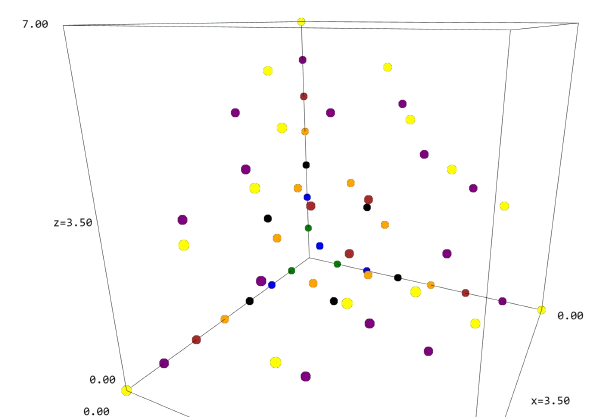
\includegraphics[height=3cm]{./Images/puntos3D.png} \\
		  \label{fig:indices}
		\end{figure}
	
  \end{frame}

  \section*{Main results}

  \begin{frame}{Biorthogonality}
	There is a relation between type I and type II MOP:
\begin{block}{Theorem 1}
  Let $\mu_1,\dots,\mu_r$ be a perfect system of $r$ 2-dimensional measures. Given $\vec n, \vec m$ multi-indices satisfying \eqref{eq:condition-type-ii} for $n$ and $m$, respectively, the following biorthogonality holds for type I and type II MOP:
  \begin{equation}
      \boxed{\prodesc{\mathbb P_{\vec n}^n}{\mathbb Q_{\vec m}} = \left\{\begin{array}{ccl}
          0_{(n+1)\times m} &   \text{ if } & \vec m \leq \vec n \\
          0_{(n+1)\times m} &   \text{ if } &  n \leq m -2 \\
          I_{n+1} & \text{ if } & n=m-1. 
      \end{array}\right.}
  \end{equation}
\end{block}
	
	
  \end{frame}

  \begin{frame}{Nearest Neighbour Relation}
	Generalisation of the TTRR satisfied by any OPS.
\begin{block}{Theorem 2}
	Let $\mu_1,\dots,\mu_r$ be a perfect system of 2-dimensional measures. Let $\vec n\in \N^r$ be a multi-index satisfying \eqref{eq:condition-type-ii} for $n\in\N$ and let us consider a path $\{\overrightarrow{m}_k:k=0,\dots,n+1\}$ where $\overrightarrow{m}_0=\vec 0, \overrightarrow{m}_n = \vec n$, each $\overrightarrow{m}_k$ satisfies \eqref{eq:condition-type-ii} for $k$ and $\overrightarrow{m}_k \leq \overrightarrow m_{k+1}$ for $k=0,\dots,n$. Then, there exist matrices $A_0,\dots,A_r$ of sizes $(n+1)\times(n-j+1)$,  $(j=0,\dots,r)$ such that
	\begin{equation}
		\label{eq:nearest-neighbour}
		x\mathbb P_{\vec n}^n = L_{{n+1},1} \mathbb P_{\overrightarrow{m}_{n+1}}^{n+1} + A_0 \mathbb P_{\vec n}^n + \sum_{j=1}^r A_j \mathbb P_{\overrightarrow{m}_{n-j}}^{n-j},
	\end{equation}
	where $L_{n+1,1}=(I_{n+1}|0_{(n+1)\times 1})$. In addition, $A_j =\nolinebreak \prodesc{x\mathbb P_{\vec n}^n}{\mathbb Q_{\overrightarrow{m}_{n-j+1}}}$.
\end{block}
  \end{frame}

  \begin{frame}{Future research topics}
	\begin{itemize}
		\item Find a Nearest Neighbour Relation for more general paths and other types of Nearest Neighbour Relations.
		\item Christoffel-Darboux formula.
		\item Look for applications to Hermite-Padé rational approximation and random matrices.
		\item Generalise existing examples to the bivariate case: Jacobi-Piñeiro, Jacobi-Angelesco, OP defined in the Simplex, etc.
		\item \dots
	  \end{itemize}
  \end{frame}

\section*{Acknowledgements}

  \begin{frame}{Acknowledgements}
	Universidad de Granada; IMAG-María de Maeztu, grant ``IMAG CEX2020--001105--M''; GOYA: ``Grupo de Ortogonalidad Y Aplicaciones'' and ``Departamento de Matemática Aplicada''.

\noindent Universidad de Almería; TAPO: ``Teoría de Aproximación y Polinomios Ortogonales'' and ``Departamento de Matemáticas''.
		\bigskip
		%& \hspace*{-5pt}
		\vspace{0.5pt}
		\centerline{
		
\includegraphics[height=1cm]{Images/ugrH} \quad
		
\includegraphics[height=1cm]{Images/ual.png} \quad
		
\includegraphics[height=1cm]{Images/goya.png}
		}
		\vspace{0.5cm}
		\centerline{
		
\includegraphics[height=1cm]{Images/IMAG} \quad
		
\includegraphics[height=1cm]{Images/maeztu} \quad
		
\includegraphics[height=1cm]{Images/tapo.png}
		}
  \end{frame}

\end{document}






